\begin{frame}[label=self]
    \frametitle{Who Am I?}   
    \raggedright
    \begin{columns}
        \begin{column}{0.8\textwidth}
            PhD candidate interested in the \hl{\textbf{intersection of radio frequency} (RF) \textbf{engineering and environmental science}}
            \begin{columns}
                \begin{column}{0.25\linewidth}
                    \begin{tcolorbox}[width=0.9\linewidth, colframe=black, arc=0pt, outer arc=0pt, opacityback=1, boxsep=1pt, left=0pt, right=0pt]
                        \centering \textit{Build \\ hardware}
                    \end{tcolorbox} %
                \end{column}
                \begin{column}{0.25\textwidth}
                    \begin{tcolorbox}[width=0.9\linewidth, colframe=black, arc=0pt, outer arc=0pt, opacityback=1, boxsep=1pt, left=0pt, right=0pt]
                        \centering \textit{Write \\ software}
                    \end{tcolorbox} 
                \end{column}
                \begin{column}{0.25\textwidth}
                    \begin{tcolorbox}[width=0.9\linewidth, colframe=black, arc=0pt, outer arc=0pt, opacityback=1, boxsep=1pt, left=0pt, right=0pt]
                        \centering \textit{Scientific \\ analysis}
                    \end{tcolorbox}    
                \end{column}
            \end{columns}
            
        \end{column}
        \begin{column}{0.2\textwidth}
            \centering
            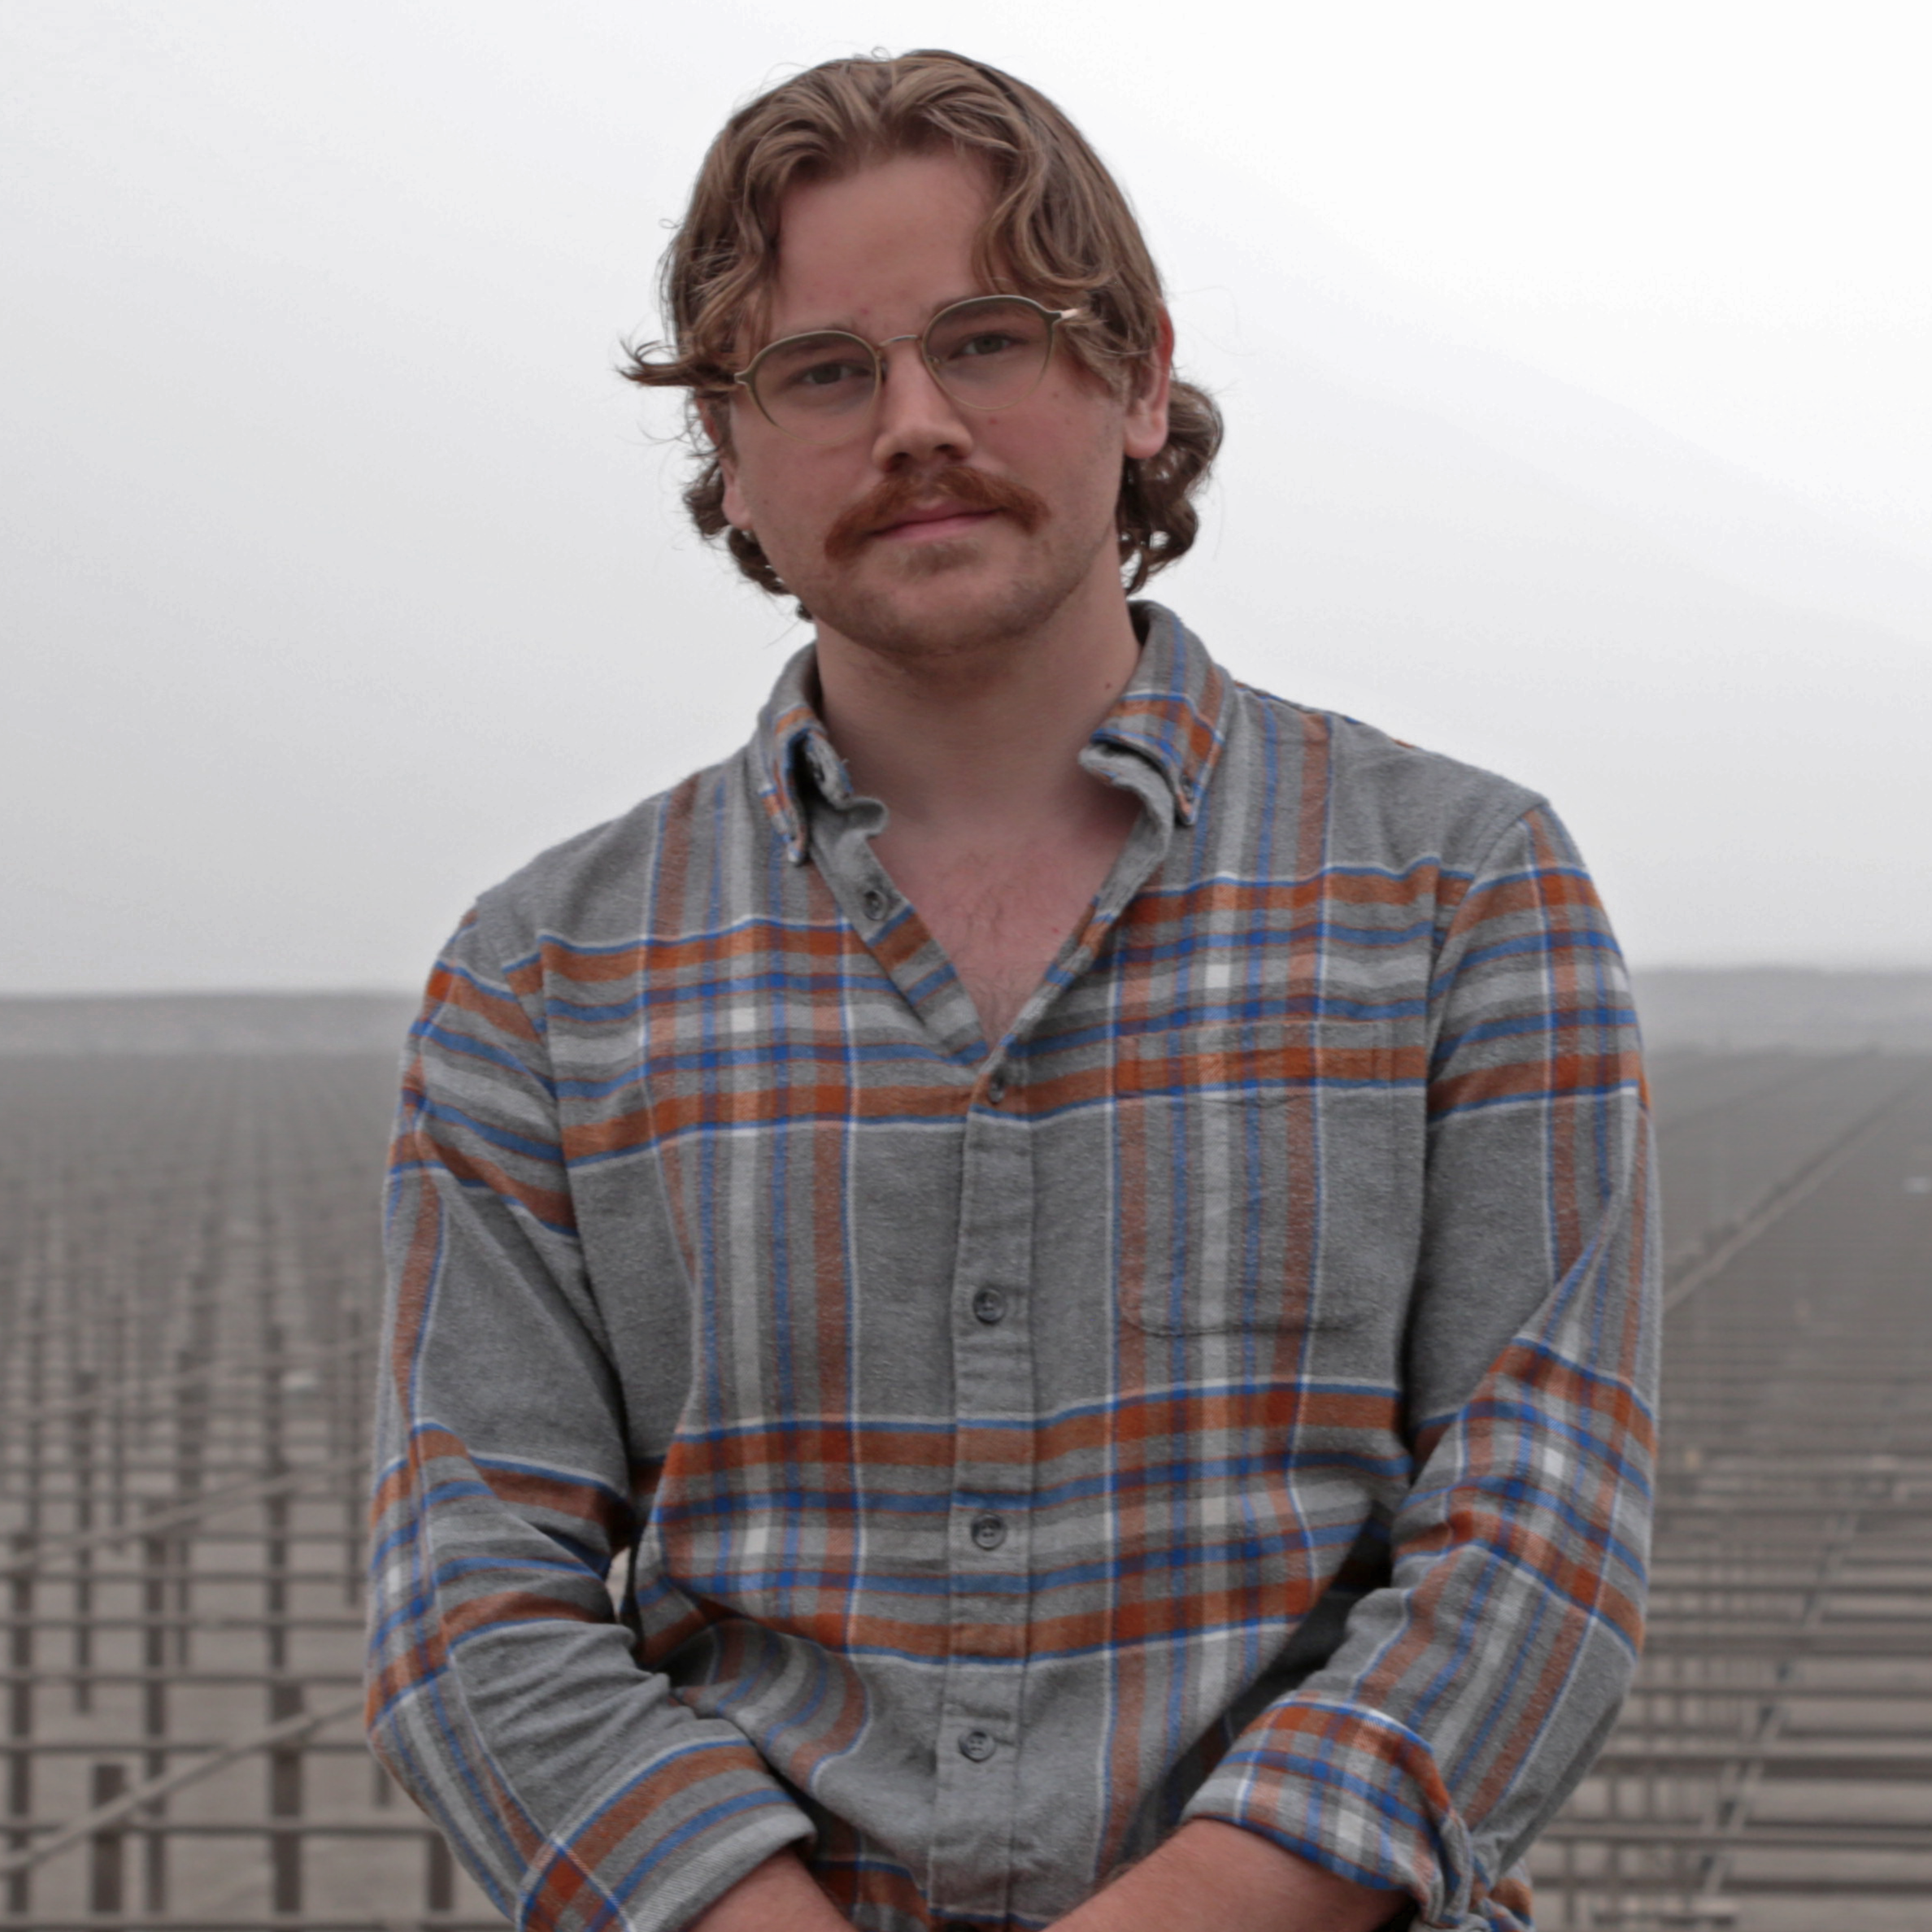
\includegraphics[width=\linewidth]{img/headshot_cropped.png}
        \end{column}
    \end{columns}
    \vspace{-\baselineskip} % 
    \begin{tabular}{p{0.35\linewidth} p{0.1\linewidth} p{0.4\linewidth}}
        \alert{Skills} &  &  \\ \arrayrulecolor{gold}\hline %
        {\setlength{\leftmargini}{1em} \begin{itemize} \tiny \vspace{-\baselineskip}%
            \item[{
\includegraphics[width=0.25cm]{img/radar_dish.pdf}}] \textit{Radar and remote sensing}
            \item[{
\includegraphics[width=0.25cm]{img/calc.pdf}}]\textit{Digital signal processing}
            \item[{
\includegraphics[width=0.25cm]{img/radio_tower.pdf}}] \textit{Radio frequency communication}
            \item[{
\includegraphics[width=0.25cm]{img/location.pdf}}]\textit{GNSS/GPS positioning systems and receivers }
        \end{itemize} }     &%
        {\setlength{\leftmargini}{1em} \begin{itemize} \tiny \vspace{-\baselineskip}%
            \item[{
\includegraphics[width=0.25cm]{img/python-logo.png}}] \textit{Python}
            \item[{
\includegraphics[width=0.25cm]{img/matlab_logo.png}}] \textit{MATLAB}
            \item[{
\includegraphics[width=0.25cm]{img/gnuradio.pdf}}] \textit{GNU Radio}
            \item[{
\includegraphics[width=0.25cm]{img/bash-logo-web.png}}] \textit{Bash}
        \end{itemize}} &  %
        {\setlength{\leftmargini}{1em} \begin{itemize} \tiny \vspace{-\baselineskip}%
            \item[{
\includegraphics[width=0.25cm]{img/sw_logo.png}}] \textit{CAD/SolidWorks}
            \item[{
\includegraphics[width=0.25cm]{img/chip.pdf}}] \textit{Embedded systems and FPGAs}
            \item[{
\includegraphics[width=0.25cm]{img/tool.pdf}}]\textit{Fabrication: machining, 3D printing, laser cutting}
        \end{itemize}}
    \end{tabular}
   {\footnotesize \begin{tabular}{lll}
        \multicolumn{3}{l}{{\normalsize \alert{Background}}} \\ \arrayrulecolor{gold}\hline
        \textbf{MS}        & Aerospace/Remote Sensing         &  \textit{CU Boulder, 2023}\\ 
        \textbf{BE} & Electrical Engineering & \textit{Dartmouth College, 2021}\\ 
        \textbf{BS} & Physics & \textit{Hobart and William Smith Colleges, 2020}\\ 
        \textbf{BS} & Chemistry &  \textit{Hobart and William Smith Colleges, 2020}       
    \end{tabular}}
    \begin{textblock*}{2cm}(13cm, 6cm)
        \centering
        
\includegraphics[width=1cm]{img/Dartmouth-Logo.png}
        
\includegraphics[width=2cm]{img/hws_logo.png}
    \end{textblock*}
\end{frame}